\renewcommand{\captiontitle}{Transformation errors}
\begin{sidewaysfigure*}
\begin{center}
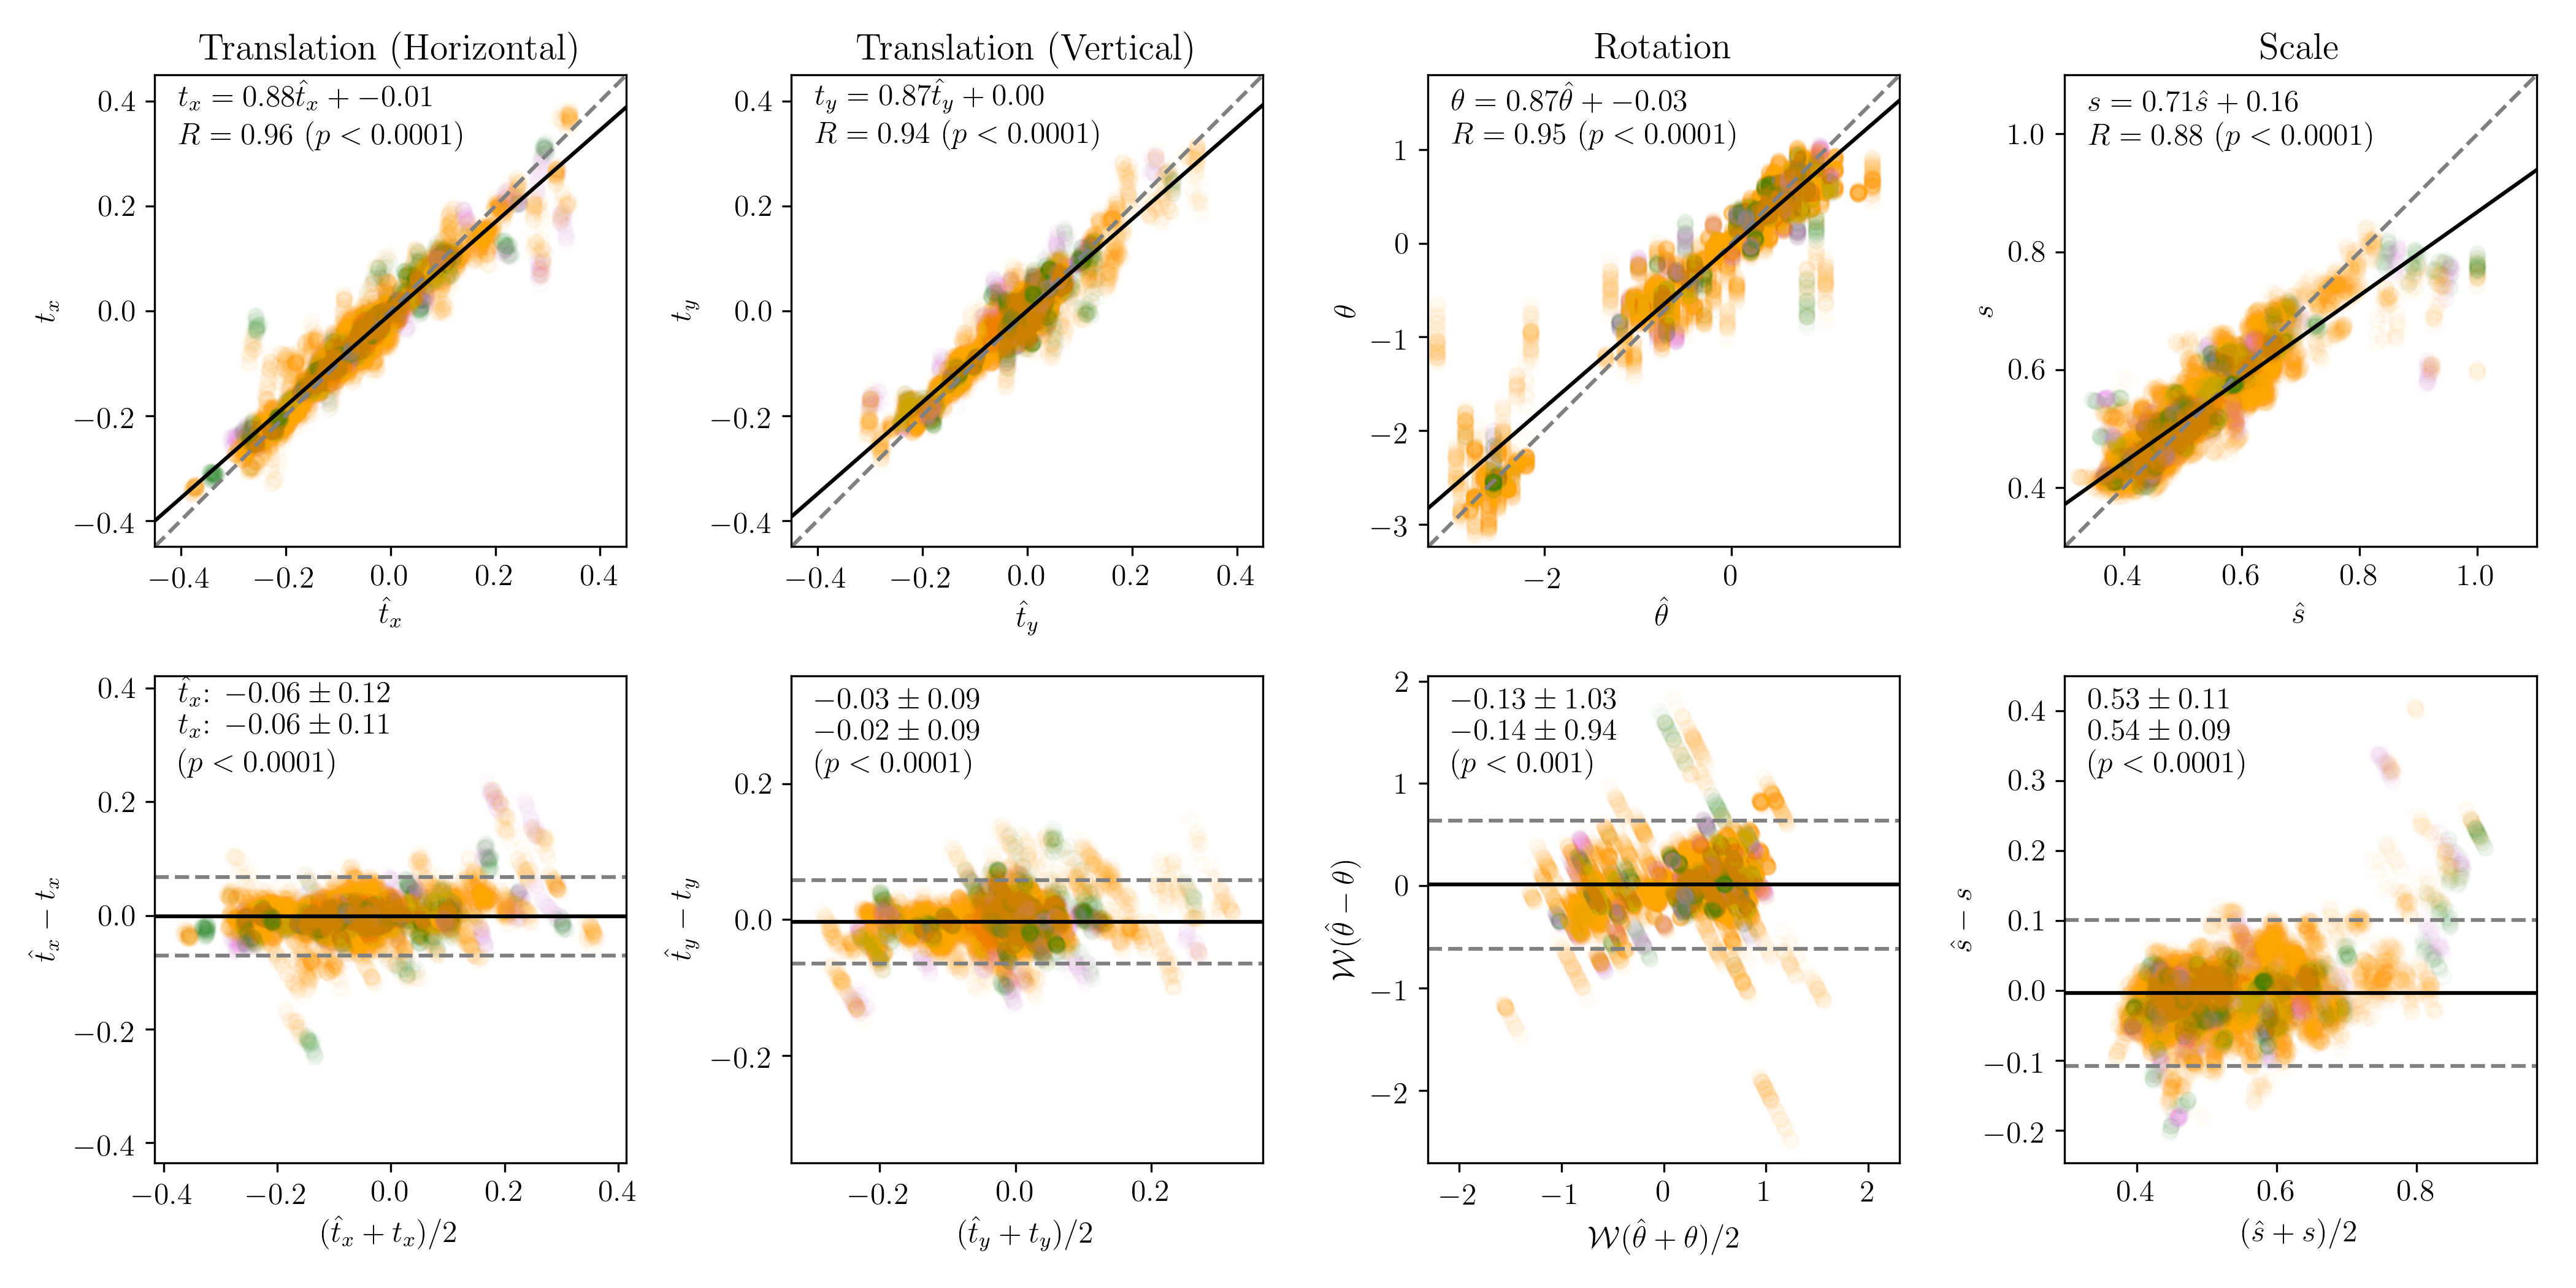
\includegraphics[width=1.0\textwidth]{./data/matrix-loss.png}
\caption[\captiontitle]{\captiontitle{}.
Correlation (top) and Bland-Altman (bottom) plots comparing predicted and ground truth transformation parameters.
\SA{}, \HLA{}, and \VLA{} errors are represented by orange, green, and purple points, respectively (points have been rendered partially translucent to aid interpretation of densely occupied regions).
In the correlation plots, the best-fit trendline is represented as a solid black line, and the ideal trendline ($y = x$) is represented as a dashed, gray line.
The equation of the trendline and the Pearson correlation coefficient $R$ are also given.
In the Bland-Altman plots, the mean difference is represented as a solid black horizontal line, and the limits $\pm 1.96$ standard deviations are represented as a dashed gray horizontal line.
}
\label{fig:matrix-loss}
\end{center}
\end{sidewaysfigure*}

